\chapter{実験}
\section{シミュレーション}
シュミレーションを利用して,設計した制御系の性能を確認する.

\subsubsection{シミュレーションソフト}
シミュレーションには数値計算ソフト「Scilab」に付属しているビジュアルモデリングソフト「Xcos」を使用する.Xcosで組み立てたブロック線図を図\ref{fig:blockXcos}に示す.この際、リフトにかかる電圧の絶対値の最大は実際と同じく12[v]に制限した.

\begin{figure}[htbp]
  \begin{center}
    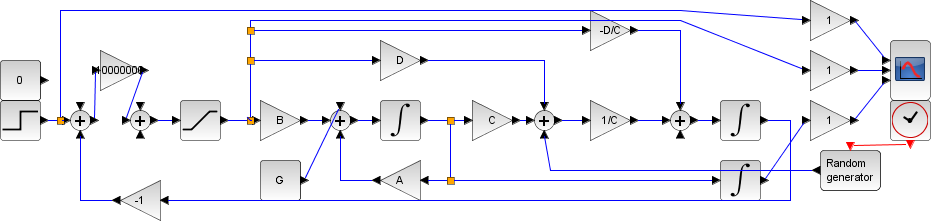
\includegraphics[width=150mm]{img/blockXcos.png}
    \end{center}
  \caption{Xcosで組み立てたブロック線図}
 \label{fig:blockXcos}
\end{figure}

\subsubsection{シミュレーション結果}
シミュレーションの結果を図\ref{fig:sim}に示す.

\begin{figure}[htbp]
 \begin{center}
    \includegraphics[width=150mm]{img/sim.bmp}
    \end{center}
  \caption{入力した目標値による電圧と位置の時間変化}
 \label{fig:sim}
\end{figure}

\subsubsection{荷重の影響}
リフトは箱を持つ個数により荷重が変化する,荷重の影響を見るためリフトの質量の値を2倍にした.その際のシミュレーション結果を図\ref{fig:sim4}に示す.

\begin{figure}[htbp]
 \begin{center}
    \includegraphics[width=150mm]{img/sim4.bmp}
    \end{center}
  \caption{荷重による影響}
 \label{fig:sim4}
\end{figure}

荷重によって電圧は2倍になったが,現在値の最終値に変化はなかった.

\subsubsection{測定誤差の影響}
実際に電流を測定した時にはノイズがあると考え,ノイズの影響を見るため電流の値に1[A]の誤差を加えてシミュレーションした.その結果を図\ref{fig:sim5}に示す.

\begin{figure}[htbp]
 \begin{center}
    \includegraphics[width=150mm]{img/sim5.bmp}
    \end{center}
  \caption{測定誤差の影響}
 \label{fig:sim5}
\end{figure}

電流の値に誤差があると,実際のリフトの速度と推定する速度にずれが生じることが分かった.

\subsubsection{測定ノイズの影響}
実際に電流を測定した時にはノイズがあると考え,ノイズの影響を見るため電流の値を分散が1[A]の正規分布になるようにした.その際のシミュレーション結果を図\ref{fig:sim2}に示す.

\begin{figure}[htbp]
 \begin{center}
    \includegraphics[width=150mm]{img/sim2.bmp}
    \end{center}
  \caption{測定ノイズの影響}
 \label{fig:sim2}
\end{figure}

電圧のグラフが激しく振動している為,塗りつぶされて見える.これは電流のノイズの影響だと考えられるが,ノイズの平均値が0ならば現在位置に影響はなかった.

\section{検出誤差の確認}
電流センサが検出する電流と実際に流れている電流に誤差があると,リフトの速度推定にも誤差が生じてしまい,時間が経つにつれリフトの位置がずれていってしまう.ここでは電流センサで検出した値がどれだけの測定誤差を持つのか確認する.

\subsubsection{使用機器}
電流センサを内蔵したモータドライバを使用した.使用したモータドライバを図\ref{fig:currentDriver}に示す.使用した機器一覧を表\ref{tab:partsCurrent}に示す.

\begin{figure}[H]
 \begin{center}
    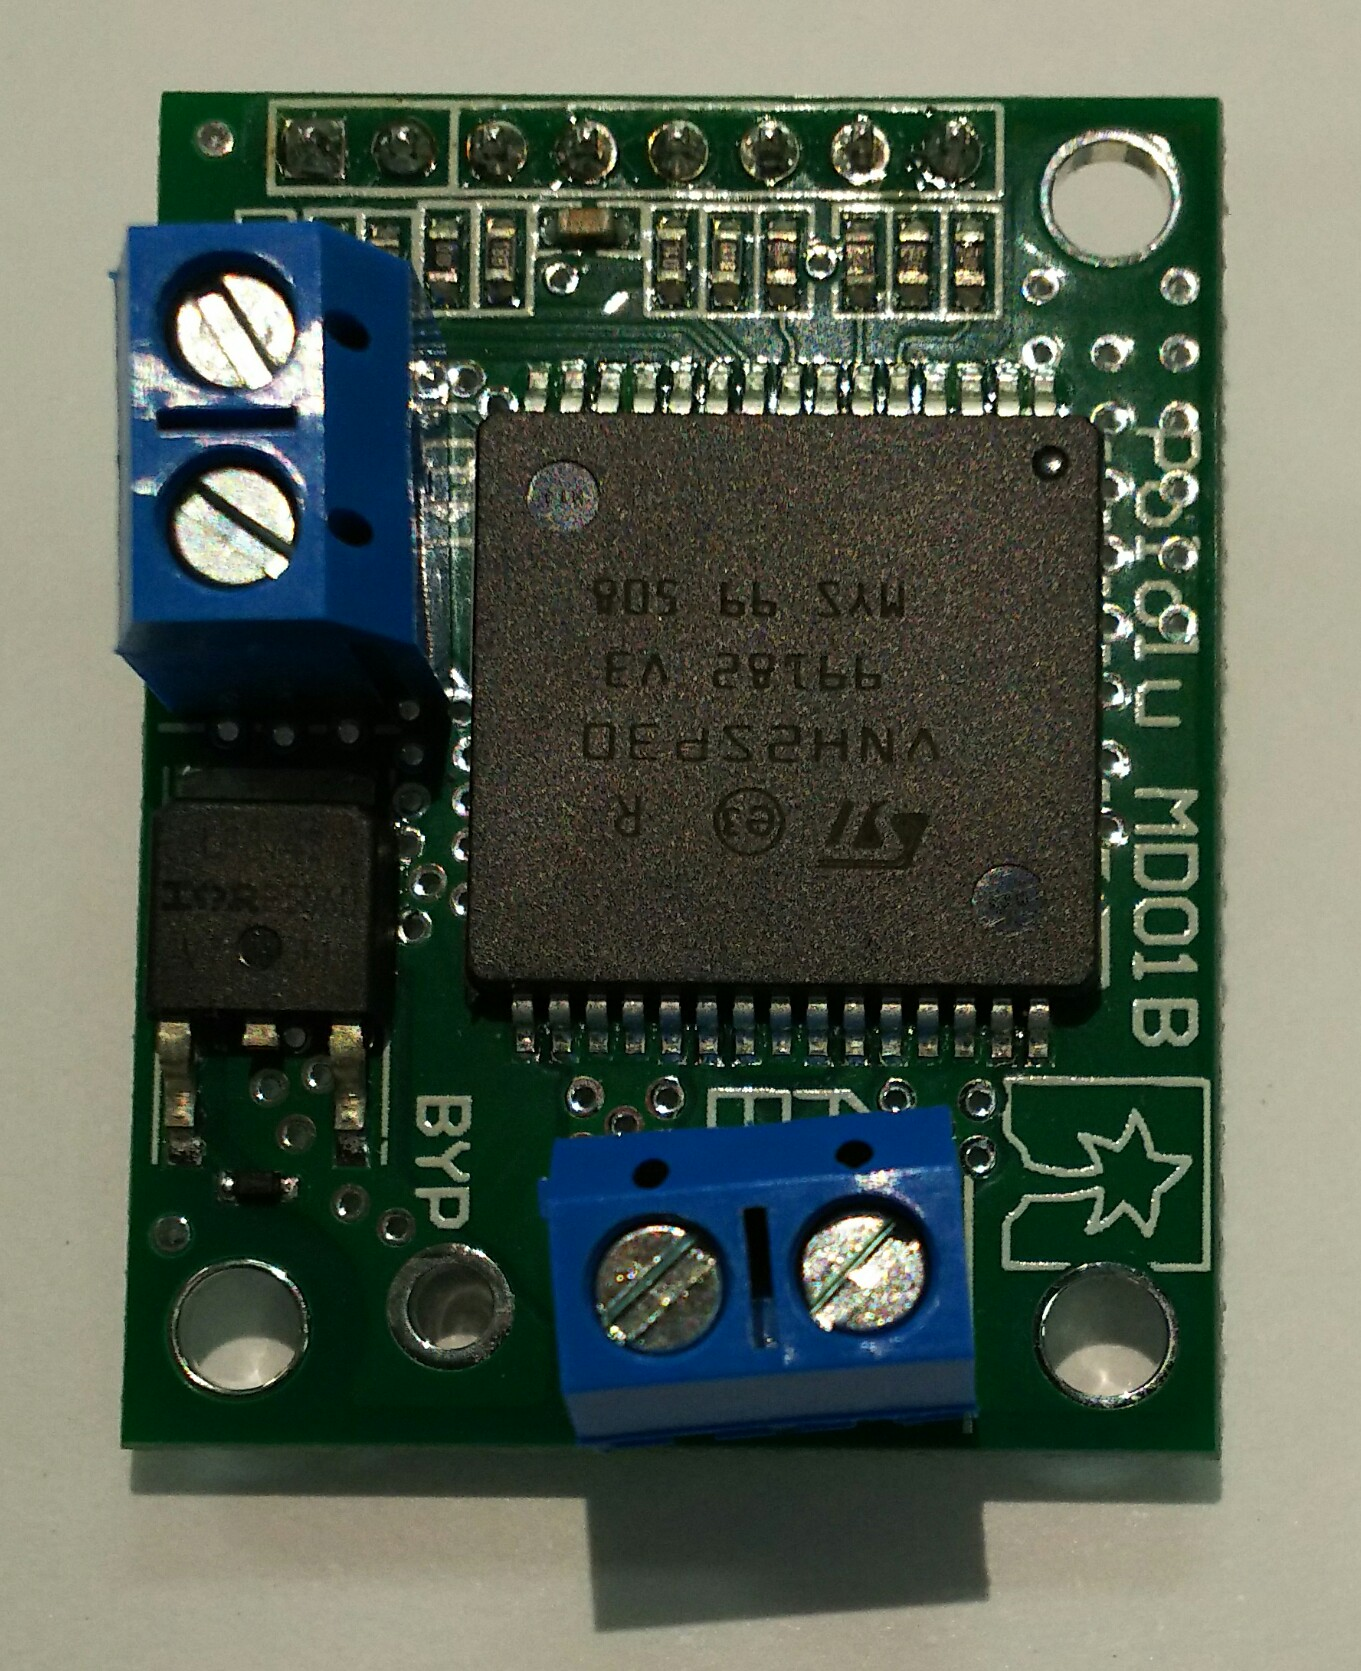
\includegraphics[width=75mm]{img/currentDriver.JPG}
    \end{center}
  \caption{電流センサ内臓モータドライバ}
 \label{fig:currentDriver}
\end{figure}

\begin{table}[H]
 \begin{center}
  \caption{搭載部品の型番とメーカ}
  \begin{tabular}[htbp]{|c|c|c|}
   \hline
   製品名&型番&メーカ \\
   \hline
   arduino&ArduinoUno&Arduino SRL\\
   \hline
   DCモータ&組み合わせモータ323726&マクソン\\
   \hline
   電流センサ内臓モータドライバ&MD01B&Pololu\\
   \hline
   テスター&VOAC86&IWATU\\
   \hline
  \end{tabular}
  \label{tab:partsCurrent}
 \end{center}
\end{table}

\subsubsection{計測方法}
\begin{enumerate}
\renewcommand{\labelenumi}{\arabic{enumi}).}
\item arduinoで,モータに常に電圧を12[v]印加するように,電流センサの値を1ミリ秒ごとに取得するようにプログラミングする.
\item 10秒以上データを記録したら,電流の平均値と分散を算出する.突入電流といい,モータに電圧を印加した直後は大きな電流が瞬間的に流れるため,しばらくたった定常状態の値を計算に使用する.
\item テスターを用いて実際の電流を計測する.
\item 電流センサでの平均値とテスターでの計測値の差を求め,ノイズの平均値とする.
\end{enumerate}

\subsubsection{電流計測}
電流を計測した結果を図\ref{fig:currentMeasurement}に示す.

\begin{figure}[H]
 \begin{center}
    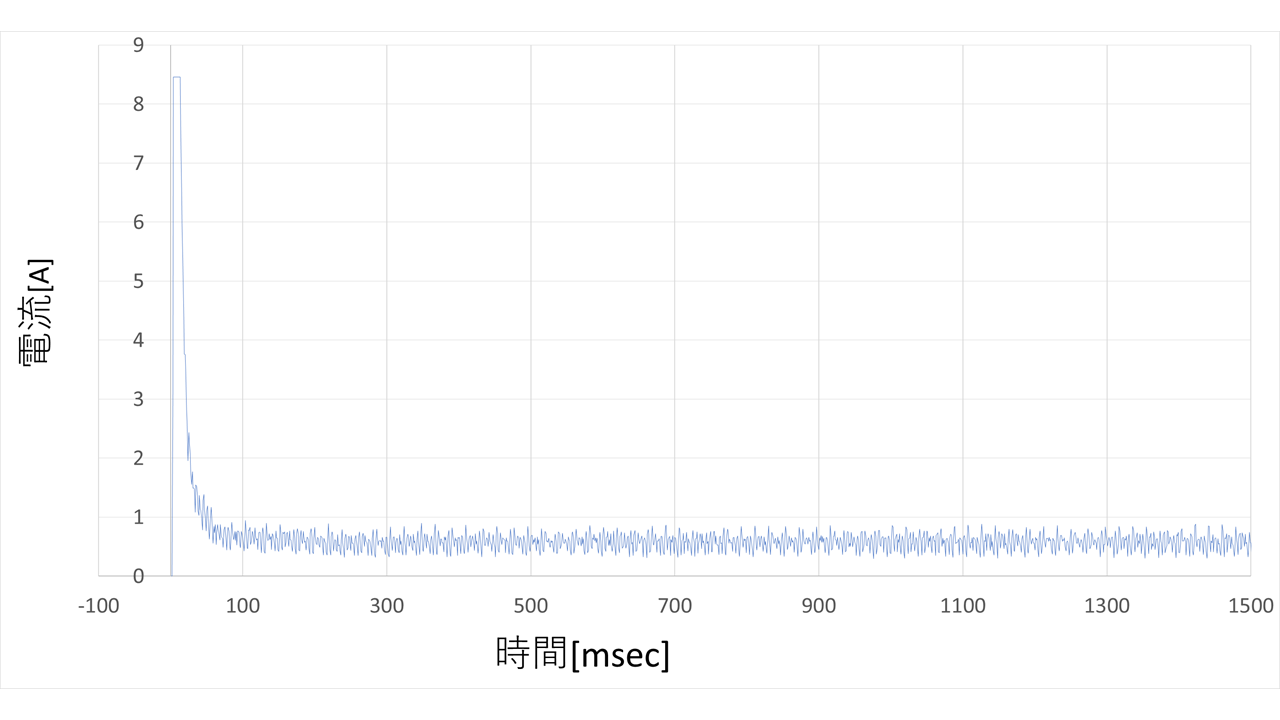
\includegraphics[width=150mm]{img/currentMeasurement.png}
    \end{center}
  \caption{電流の時間変化}
 \label{fig:currentMeasurement}
\end{figure}

検出した電流の平均は0.575[A],ノイズの分散は0.016[A],テスターでの計測結果は0.232[A]となった.よってノイズの平均は0.343[A]となった.
\\
モータに印加する電圧を負にして,逆転させた場合の計測結果を図\ref{fig:currentMeasurement2}に示す.

\begin{figure}[H]
 \begin{center}
    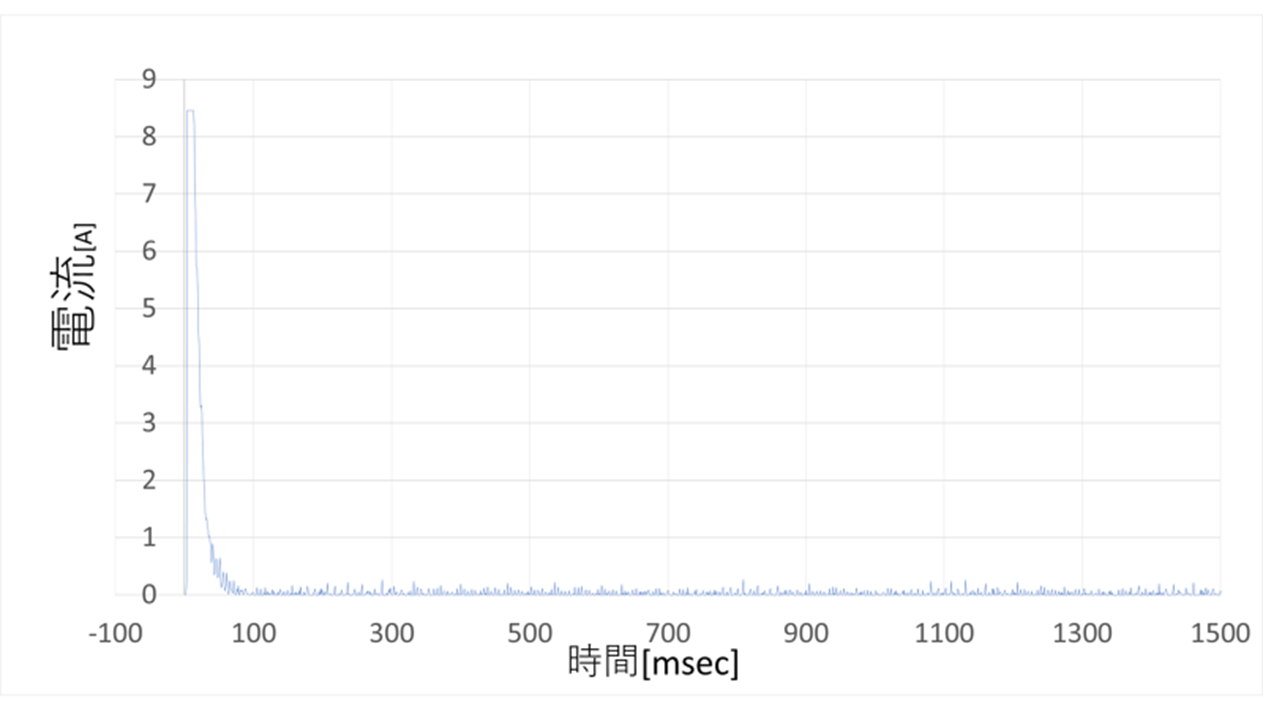
\includegraphics[width=150mm]{img/currentMeasurement2.png}
    \end{center}
  \caption{電流の時間変化}
 \label{fig:currentMeasurement2}
\end{figure}

検出した電流の平均は0.027[A],ノイズの分散は0.002[A]となった.よってノイズの平均は-0.205[A]となった.
%オシロの図とメーカ名もいるので書いといて
正転時と逆転時に電圧の違いが表れたが,arduinoのAD変換器に原因がある可能性を考え,オシロスコープで電流センサから出力される電圧を直接観察した.その結果を図\ref{fig:osiro_0},図\ref{fig:osiro_seiten},図\ref{fig:osiro_gyakuten}に示す.

\begin{figure}[htbp]
 \begin{center}
    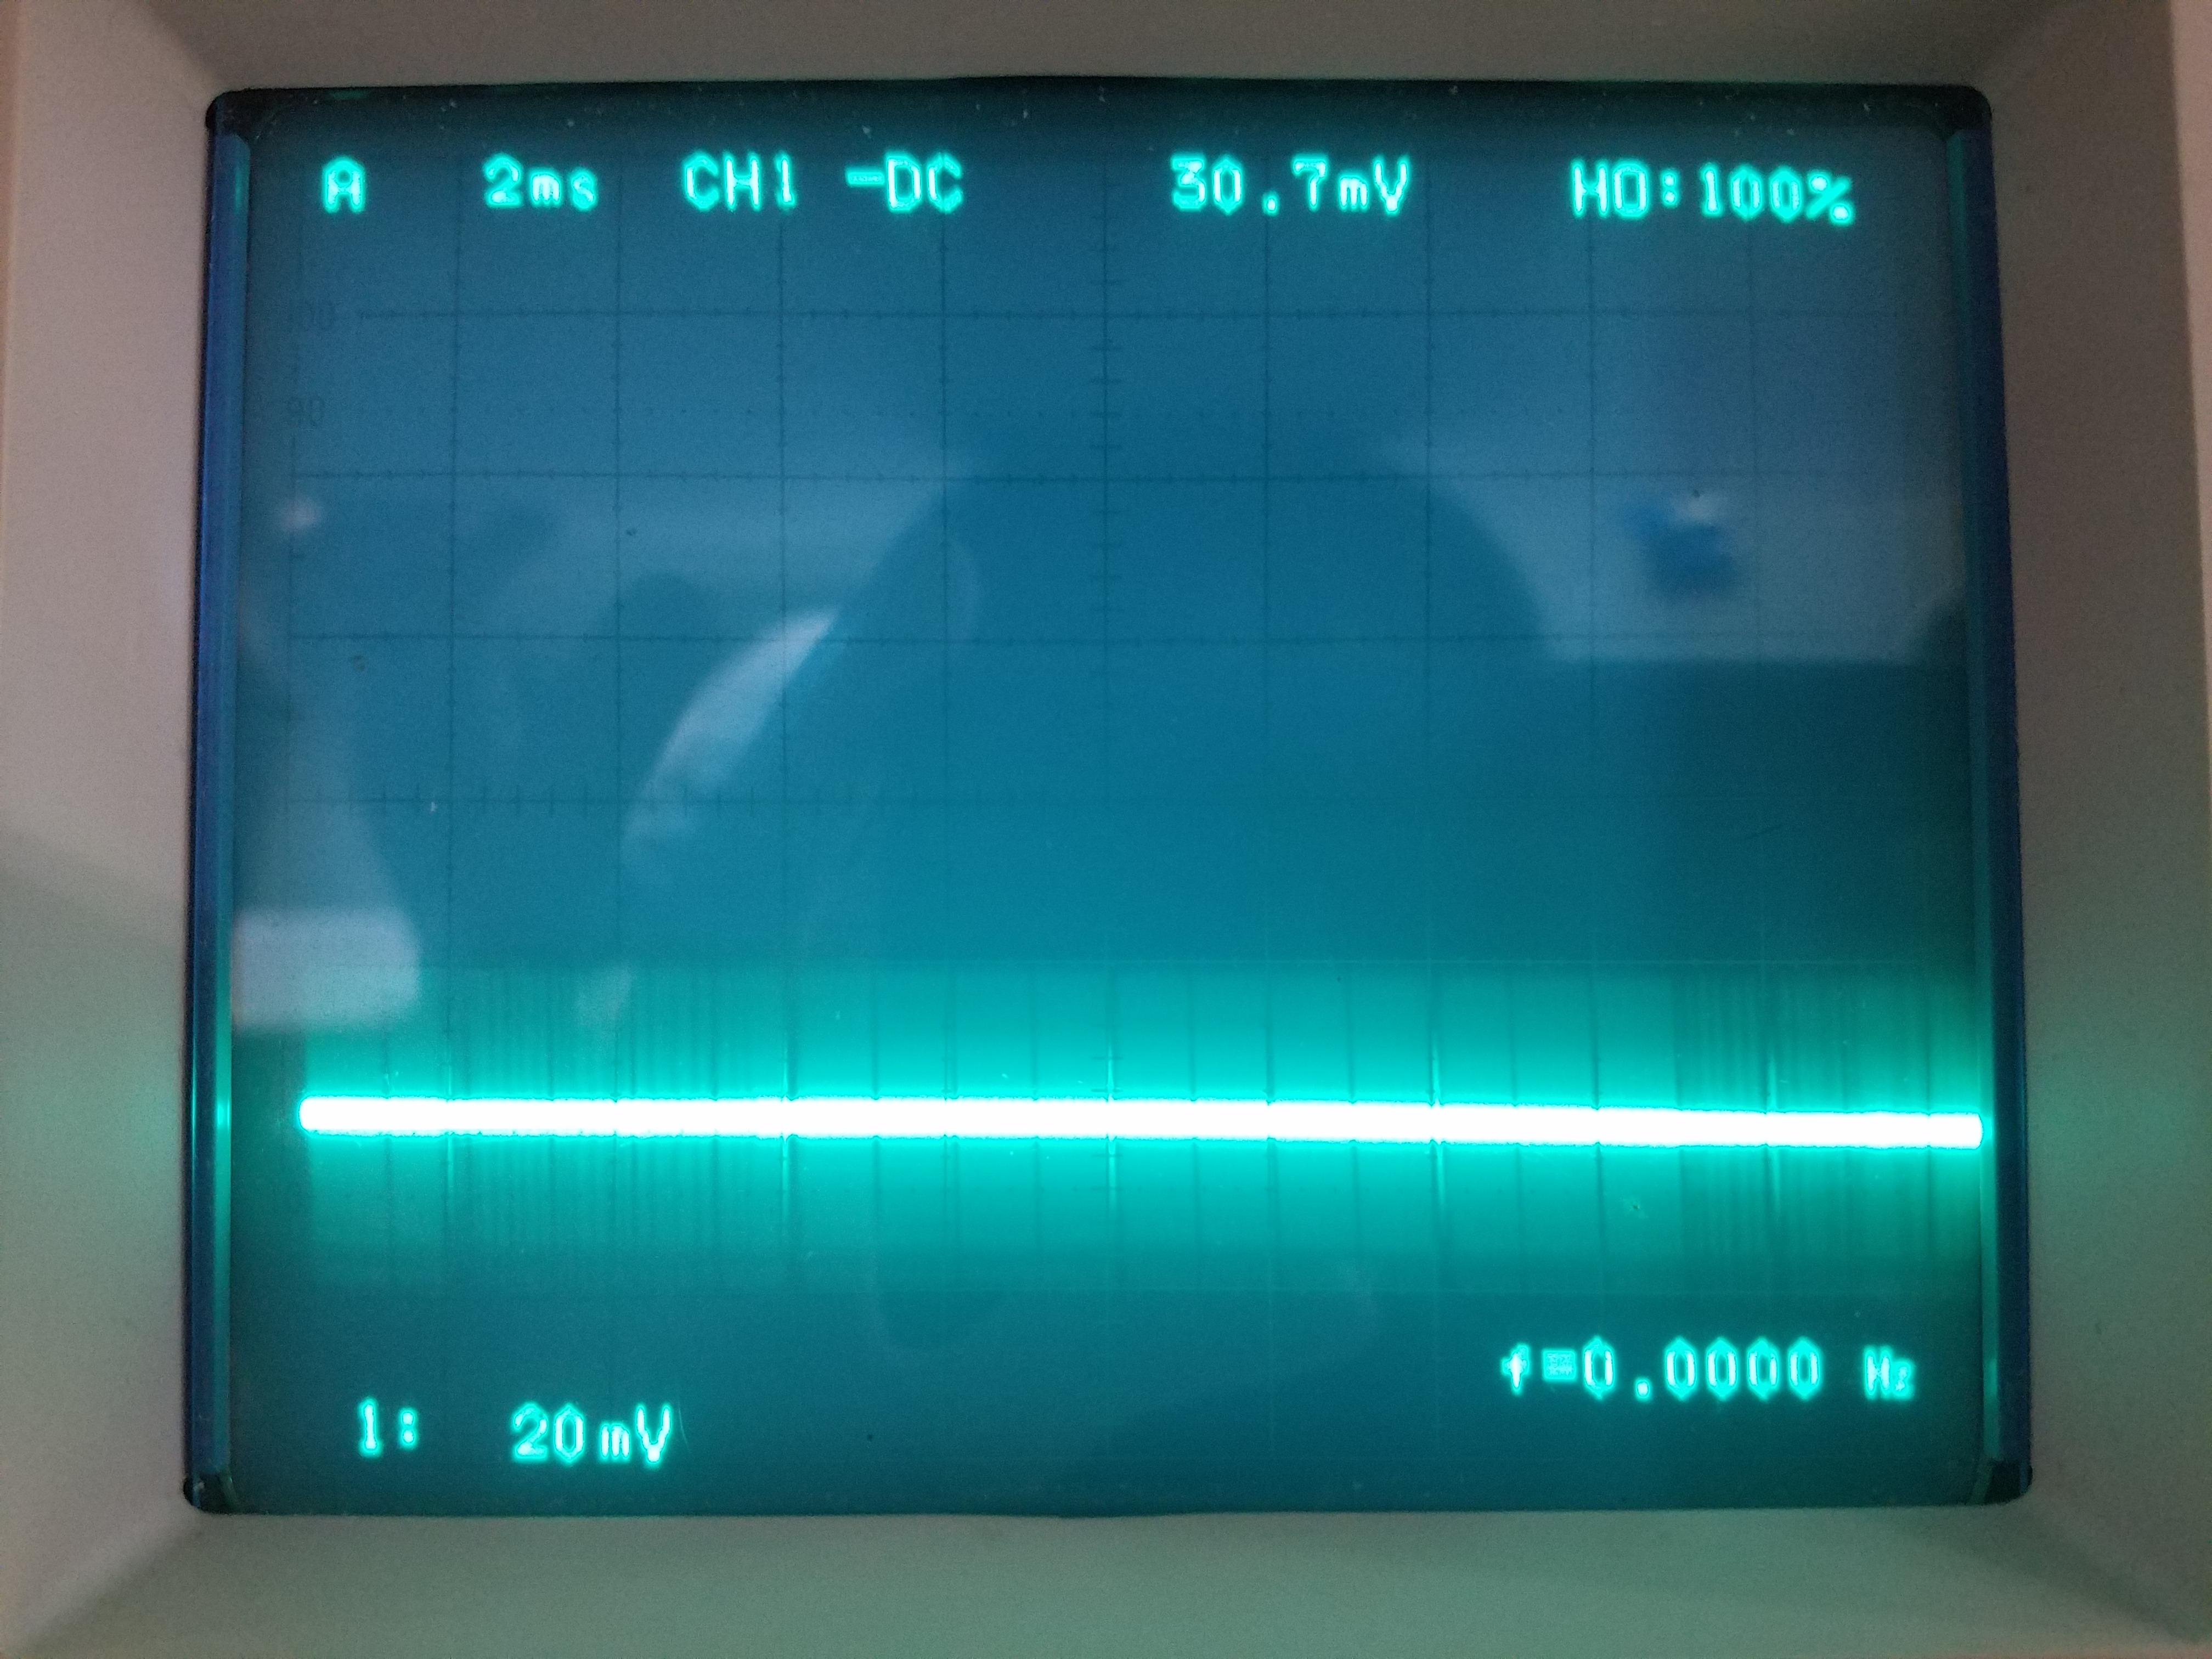
\includegraphics[width=100mm]{img/osiro_0.jpg}
    \end{center}
  \caption{無回転時の電圧}
 \label{fig:osiro_0}
\end{figure}

\begin{figure}[htbp]
 \begin{center}
    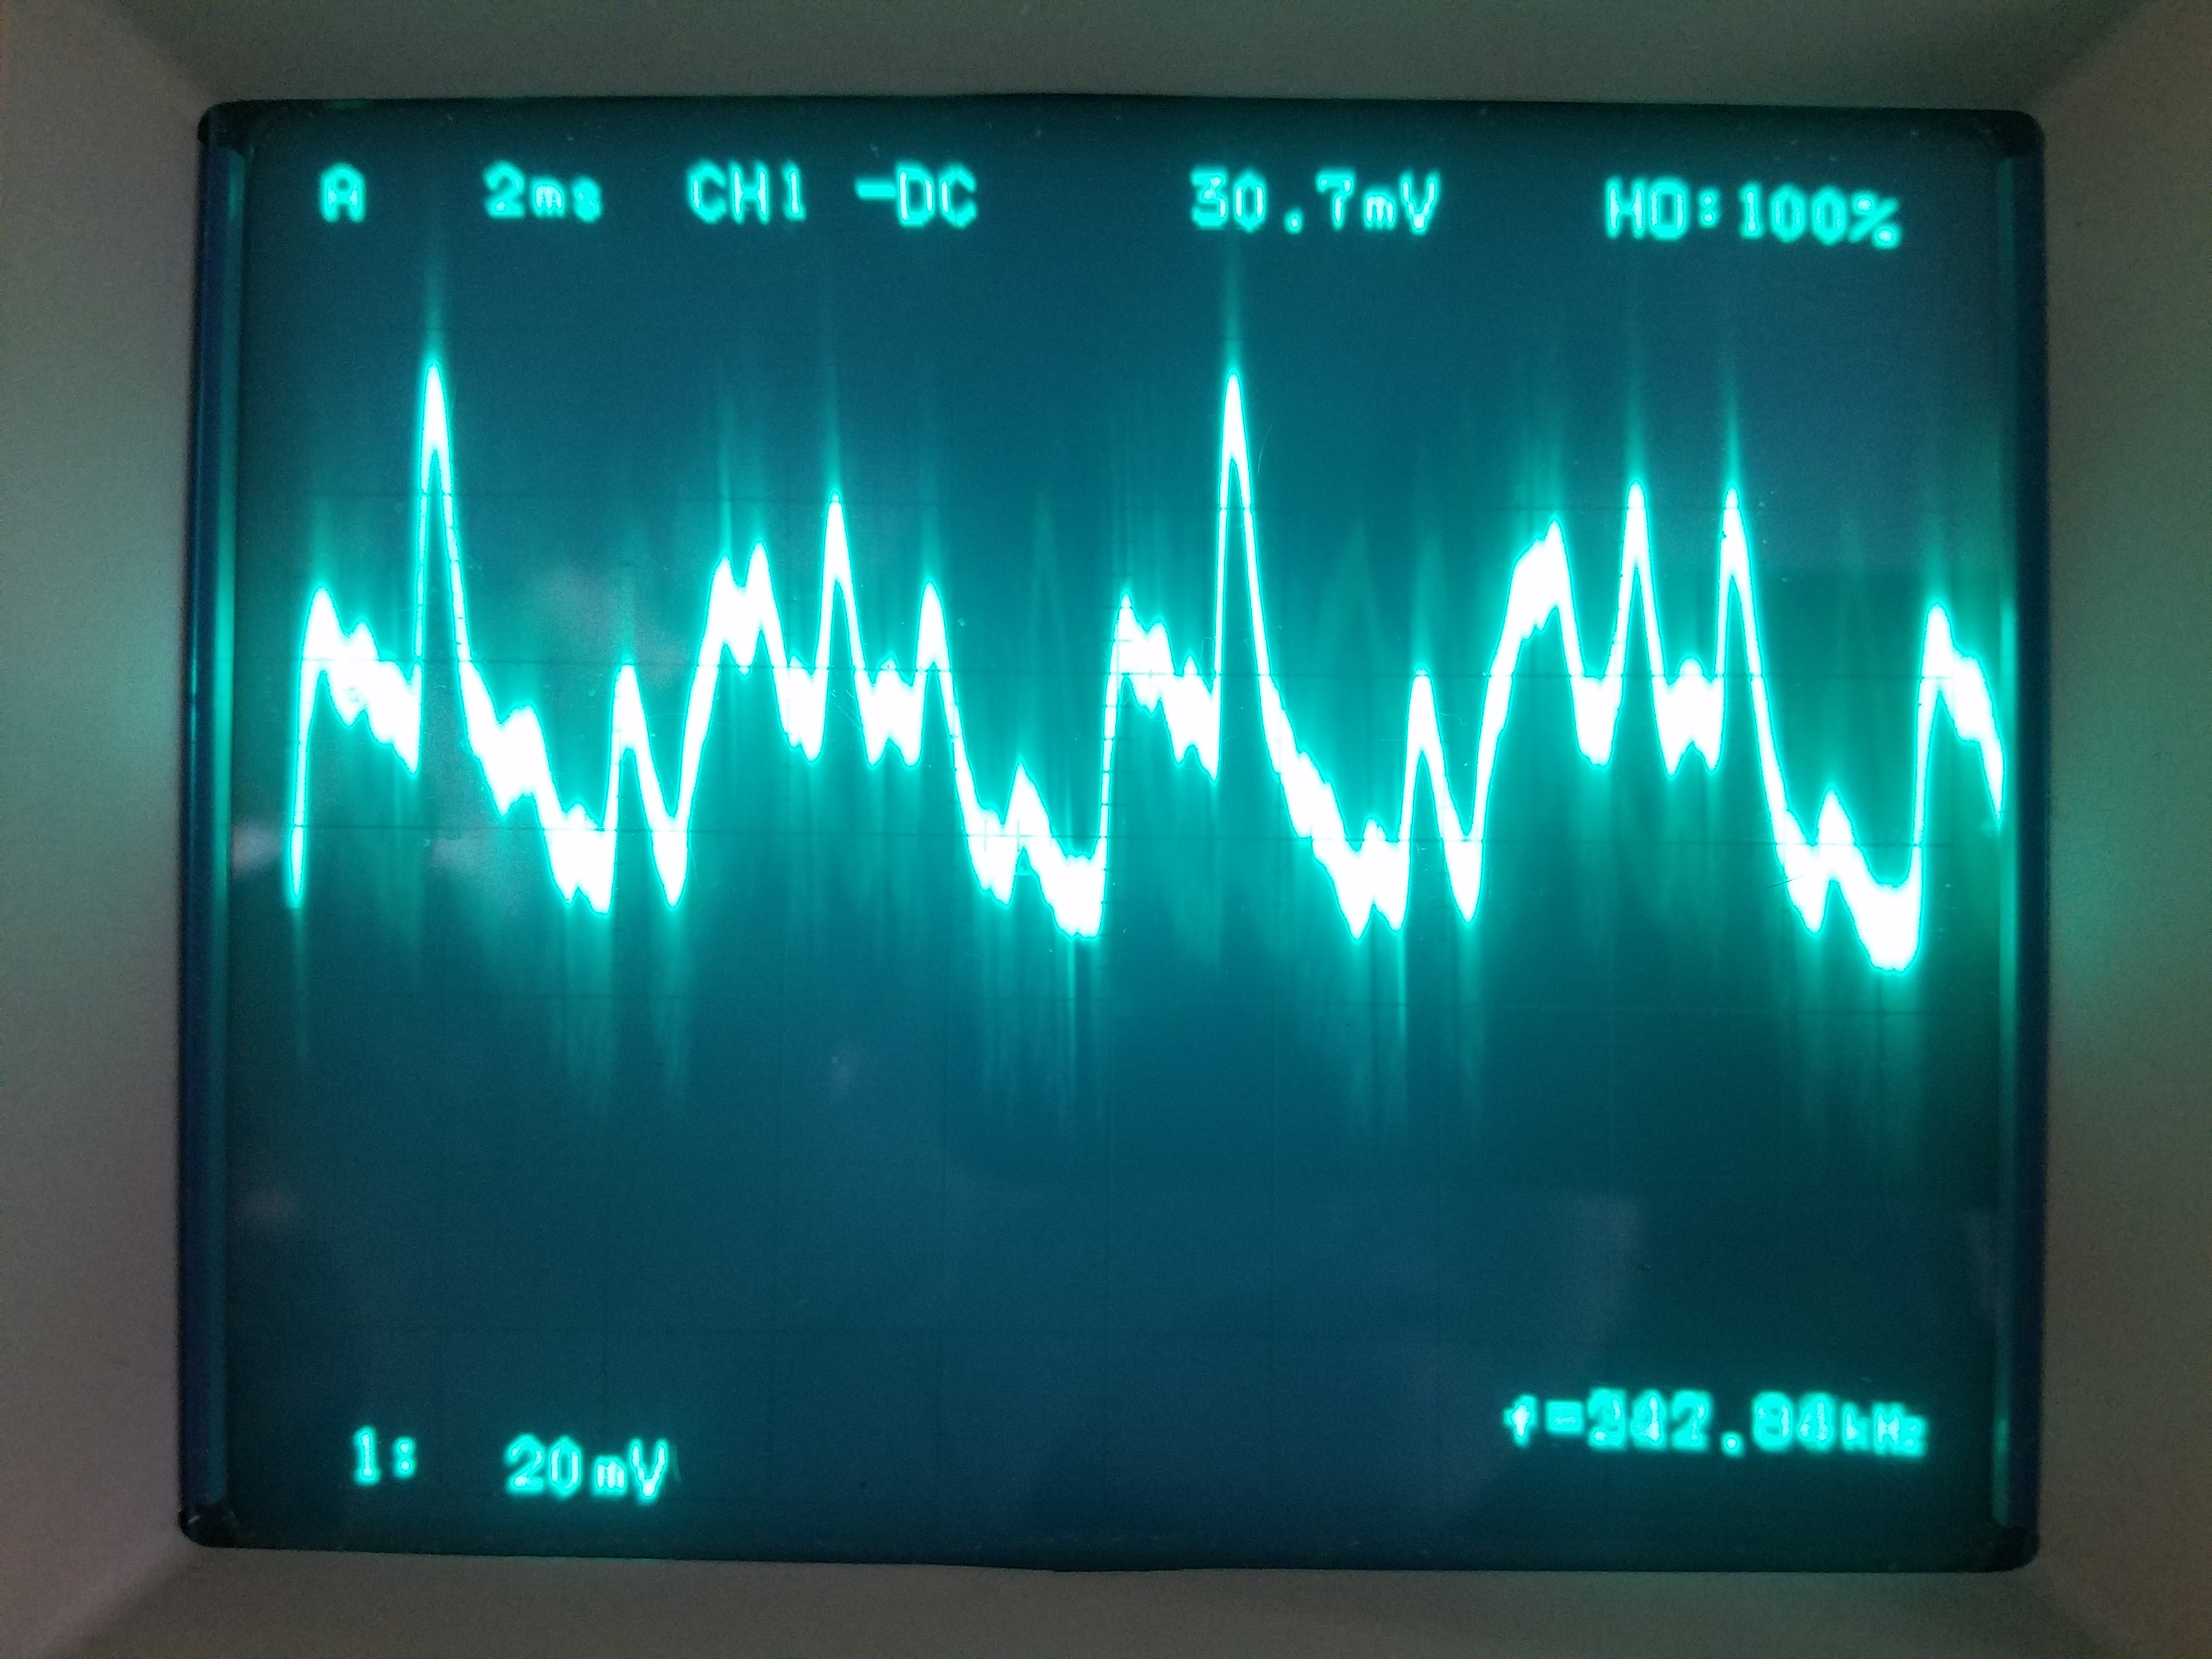
\includegraphics[width=100mm]{img/osiro_seiten.jpg}
    \end{center}
  \caption{正転時の電圧}
 \label{fig:osiro_seiten}
\end{figure}

\begin{figure}[htbp]
 \begin{center}
    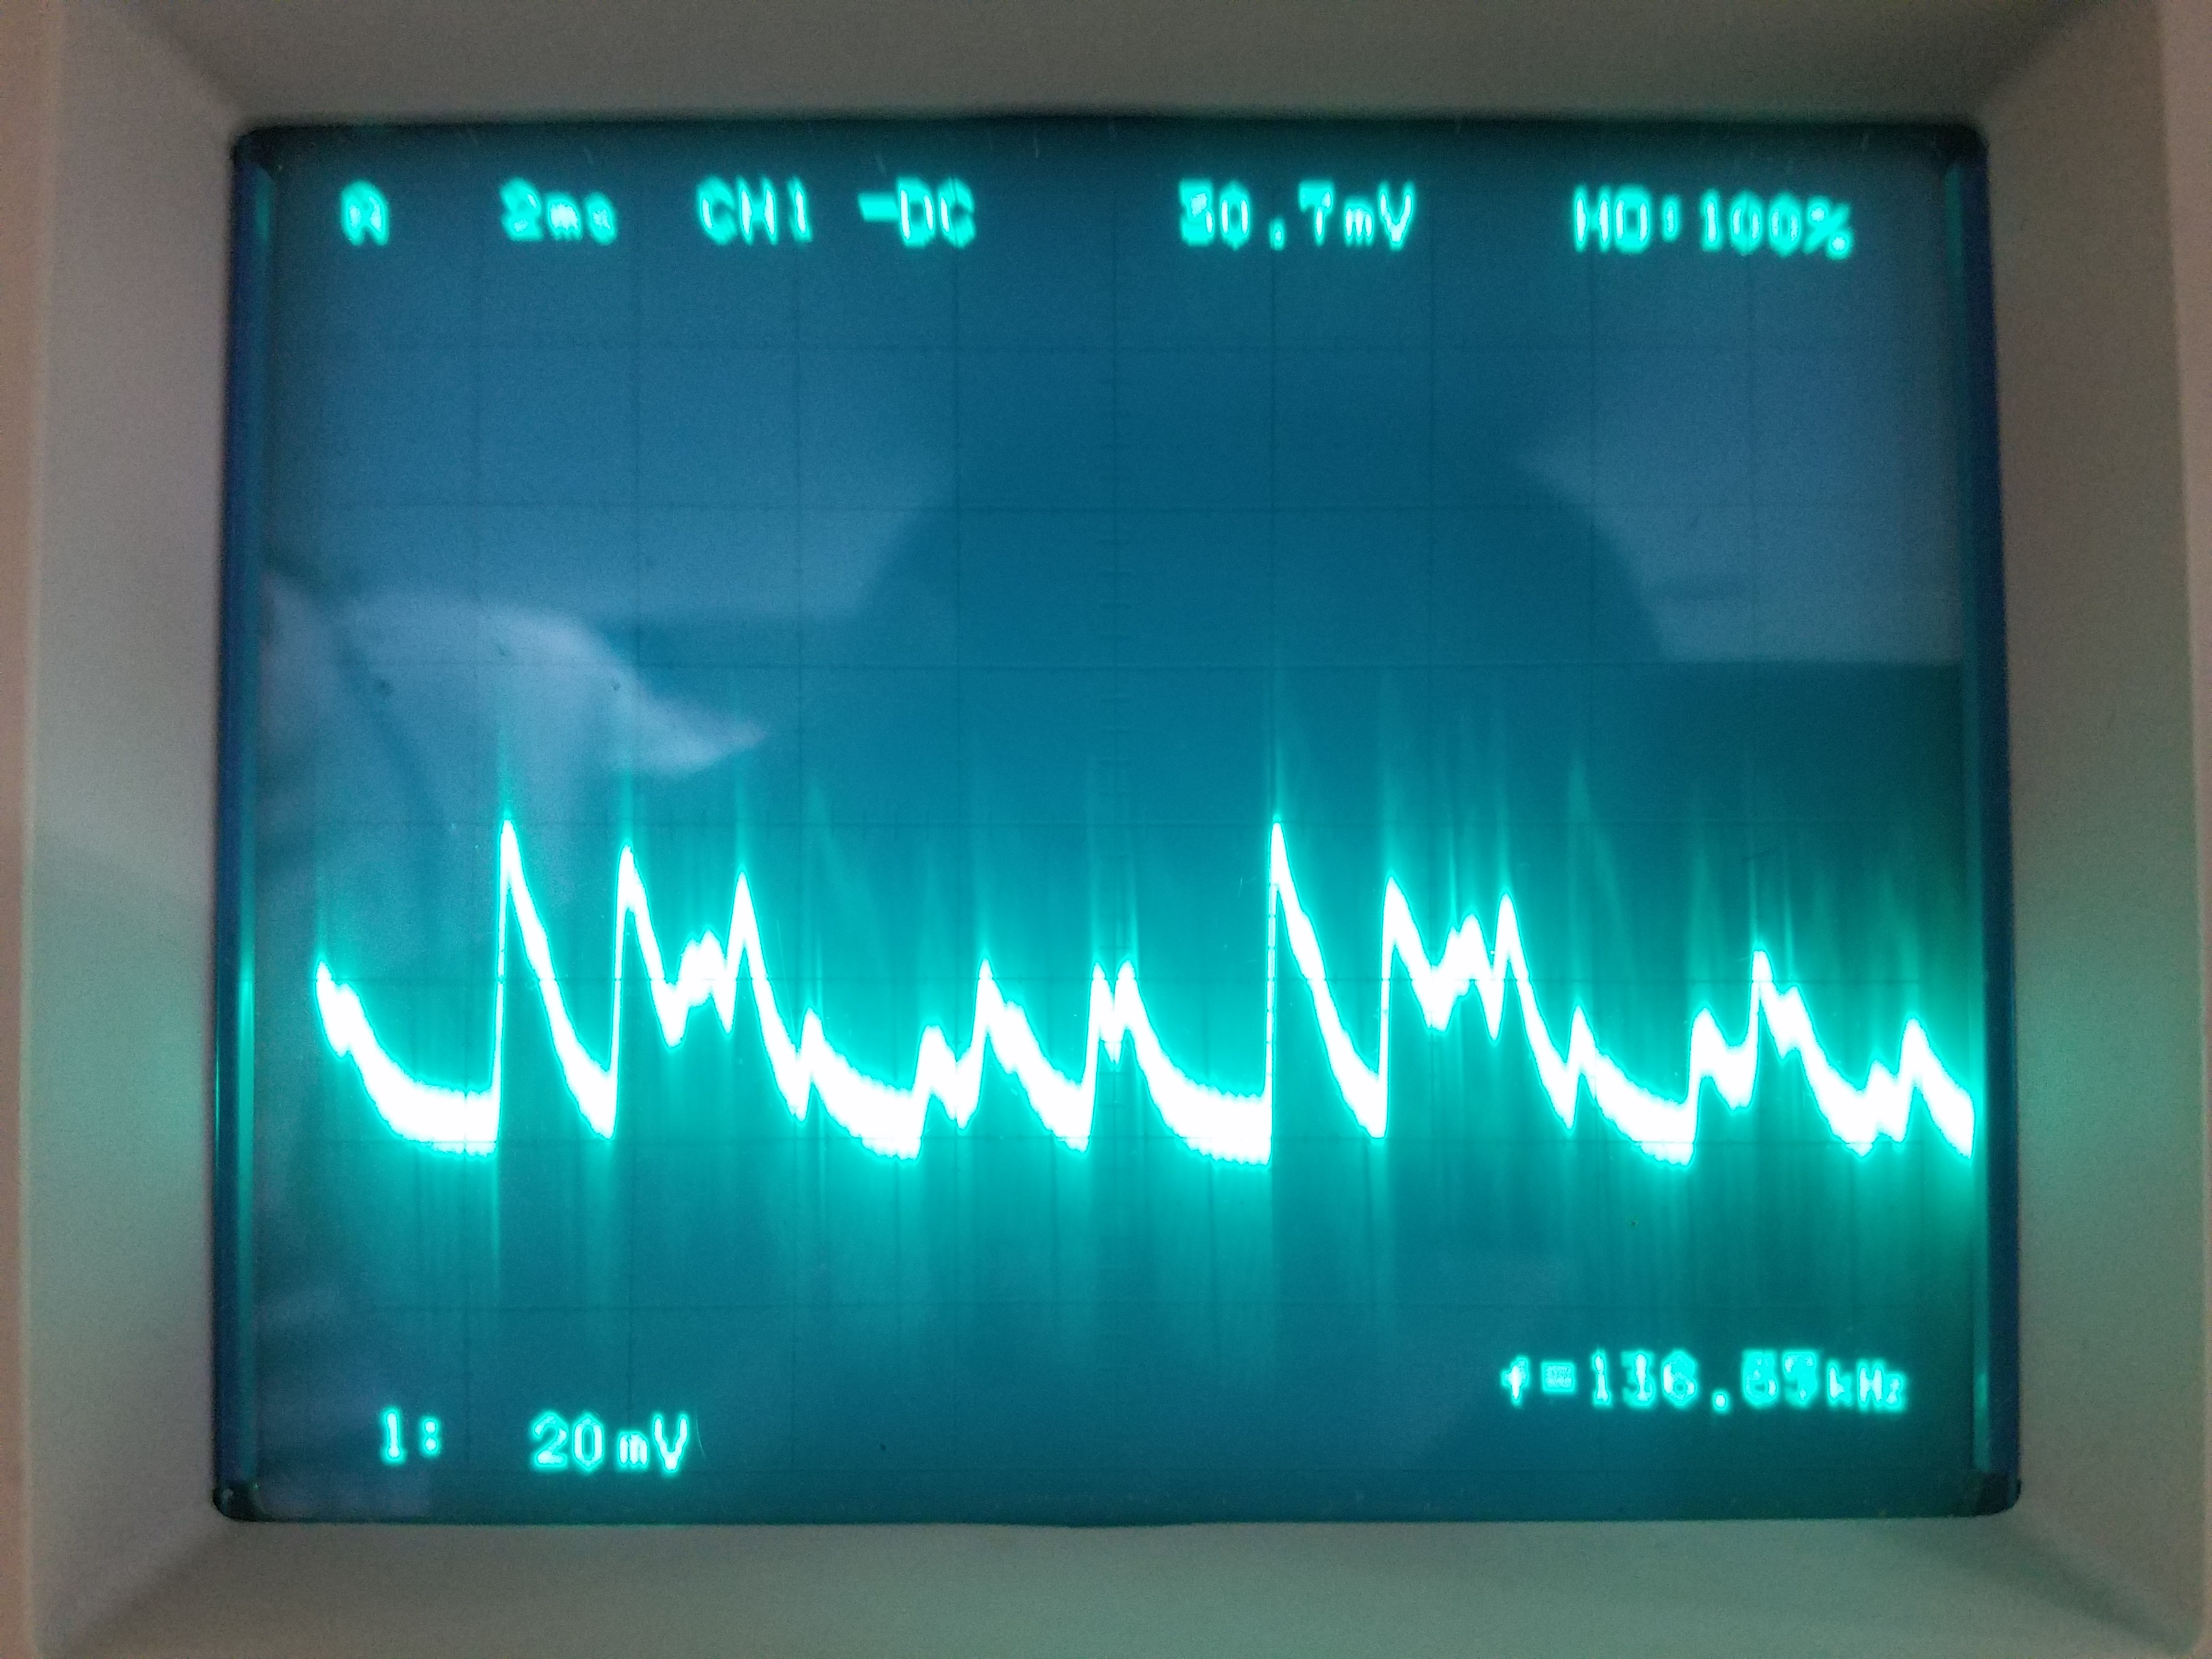
\includegraphics[width=100mm]{img/osiro_gyakuten.jpg}
    \end{center}
  \caption{逆転時の電圧}
 \label{fig:osiro_gyakuten}
\end{figure}







%図入れといて
オシロスコープでの観察でも電圧の値に差がみられた.
